\documentclass[aspectratio=169,10pt]{beamer}

% Theme & Styling
\usetheme{Madrid}
\usecolortheme{whale}

% ITB Color Palette
\definecolor{ITBblue}{RGB}{0, 75, 141}
\definecolor{ITBgold}{RGB}{200, 150, 40}
\setbeamercolor{structure}{fg=ITBblue}
\setbeamercolor{title}{fg=white,bg=ITBblue}
\setbeamercolor{frametitle}{fg=white,bg=ITBblue}
\setbeamercolor{block title}{fg=white,bg=ITBblue}
\setbeamercolor{block body}{bg=ITBblue!8}

% Packages
\usepackage[utf8]{inputenc}
\usepackage{amsmath,amssymb}
\usepackage{graphicx}
\usepackage{hyperref}
\usepackage{multimedia}

\title[MA1101 Matematika I]{MA1101 Matematika I --- Bab 2: Turunan}
\subtitle{Subtopik 2.9: Diferensial dan Hampiran (\textit{Differentials and Approximations})}
\author[FMIPA ITB]{Tim Pengajar MA1101}
\institute[ITB]{Fakultas Matematika dan Ilmu Pengetahuan Alam\\Institut Teknologi Bandung}
\date{Semester 1 Tahun Akademik 2026/2027}

\begin{document}

% -------------------------------------------------------------
% Slide 1: Judul
% -------------------------------------------------------------
\begin{frame}
    \titlepage
\end{frame}

% -------------------------------------------------------------
% Slide 2: Motivasi & Tantangan Sokratik (The Pique)
% -------------------------------------------------------------
\begin{frame}{Tantangan Awal: Menghitung Nilai Rumit Tanpa Kalkulator}
    \begin{columns}[T]
        \begin{column}{0.55\textwidth}
            \begin{block}{Motivasi Utama}
                \begin{itemize}
                    \item \textbf{Komputasi Manual}: Menaksir nilai rumit ($\sqrt{4.08}$, $\sqrt[3]{28}$, $\cos(29^\circ)$) secara cepat tanpa alat hitung digital.
                    \item \textbf{Toleransi Alat Ukur}: Menaksir bagaimana galat pengukuran fisik ($r = 10 \pm 0.1\text{ cm}$) merambat ke perhitungan volume atau luas.
                \end{itemize}
            \end{block}

            \vspace{0.15cm}
            \begin{alertblock}{Pertanyaan Sokratik}
                Garis lurus adalah kurva paling sederhana ($y = mx + c$).\\
                Dapatkah kita menggantikan kurva lengkung yang rumit dengan \textbf{garis singgung} di sekitar titik acuan untuk mempermudah perhitungan?
            \end{alertblock}
        \end{column}

        \begin{column}{0.42\textwidth}
            \centering
            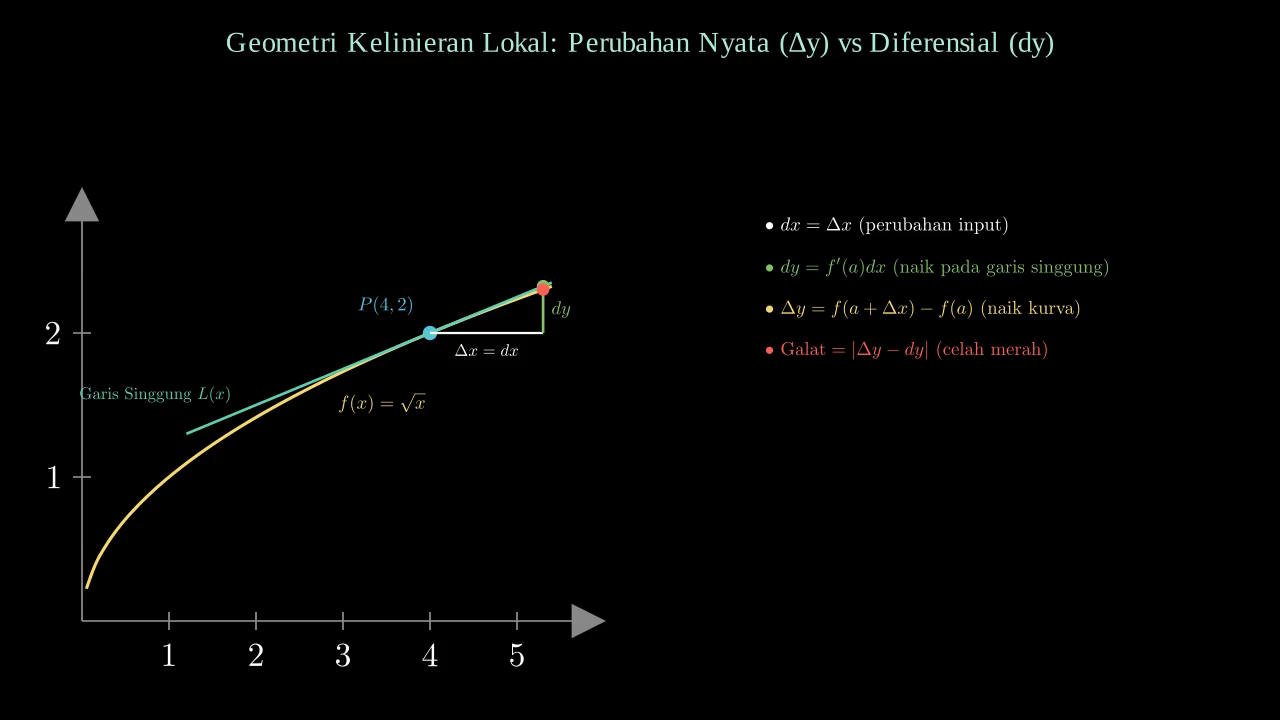
\includegraphics[width=\textwidth]{keyframe_diferensial.png}\\
            \vspace{0.1cm}
            {\scriptsize \textit{Kelinieran Lokal: Garis singgung mendekati kurva di sekitar titik $P(4, 2)$}}
        \end{column}
    \end{columns}
\end{frame}

% -------------------------------------------------------------
% Slide 3: Konsep Geometris: \Delta y vs dy
% -------------------------------------------------------------
\begin{frame}{Konsep Geometris: Perubahan Nyata ($\Delta y$) vs Diferensial ($dy$)}
    \begin{columns}[T]
        \begin{column}{0.49\textwidth}
            \begin{block}{1. Perubahan Input}
                Misalkan $x$ berubah dari $a$ ke $a + \Delta x$:
                \[
                    \mathbf{dx = \Delta x} \quad \text{(diferensial variabel bebas)}
                \]
            \end{block}

            \begin{block}{2. Perubahan Nyata ($\Delta y$) vs Diferensial ($dy$)}
                \begin{itemize}
                    \item \textbf{Kenaikan Nyata pada Kurva}:
                    \[
                        \mathbf{\Delta y = f(a + \Delta x) - f(a)}
                    \]
                    \item \textbf{Kenaikan pada Garis Singgung}:
                    \[
                        \mathbf{dy = f'(a)\,dx}
                    \]
                \end{itemize}
            \end{block}
        \end{column}

        \begin{column}{0.49\textwidth}
            \begin{alertblock}{Analisis Galat Hampiran}
                Selisih kenaikan kurva dan garis singgung:
                \[
                    \text{Galat Mutlak} = |\Delta y - dy|
                \]
            \end{alertblock}

            \begin{exampleblock}{Teorema Kelinieran Lokal}
                Ketika $\Delta x \to 0$, celah galat menyusut \textbf{jauh lebih cepat} daripada $\Delta x$:
                \[
                    \lim_{\Delta x \to 0} \frac{\Delta y - dy}{\Delta x} = 0 \implies \mathbf{\Delta y \approx dy}
                \]
                Garis singgung adalah \textbf{hampiran linier terbaik}!
            \end{exampleblock}
        \end{column}
    \end{columns}
\end{frame}

% -------------------------------------------------------------
% Slide 4: Animasi Video Interaktif
% -------------------------------------------------------------
\begin{frame}{Simulasi Dinamis: Garis Singgung \& Diferensial}
    \centering
    % Embedded video untuk presenter (Pympress / PDFPC / Okular)
    \movie[width=9.6cm,height=5.4cm,poster,showcontrols=true]{%
        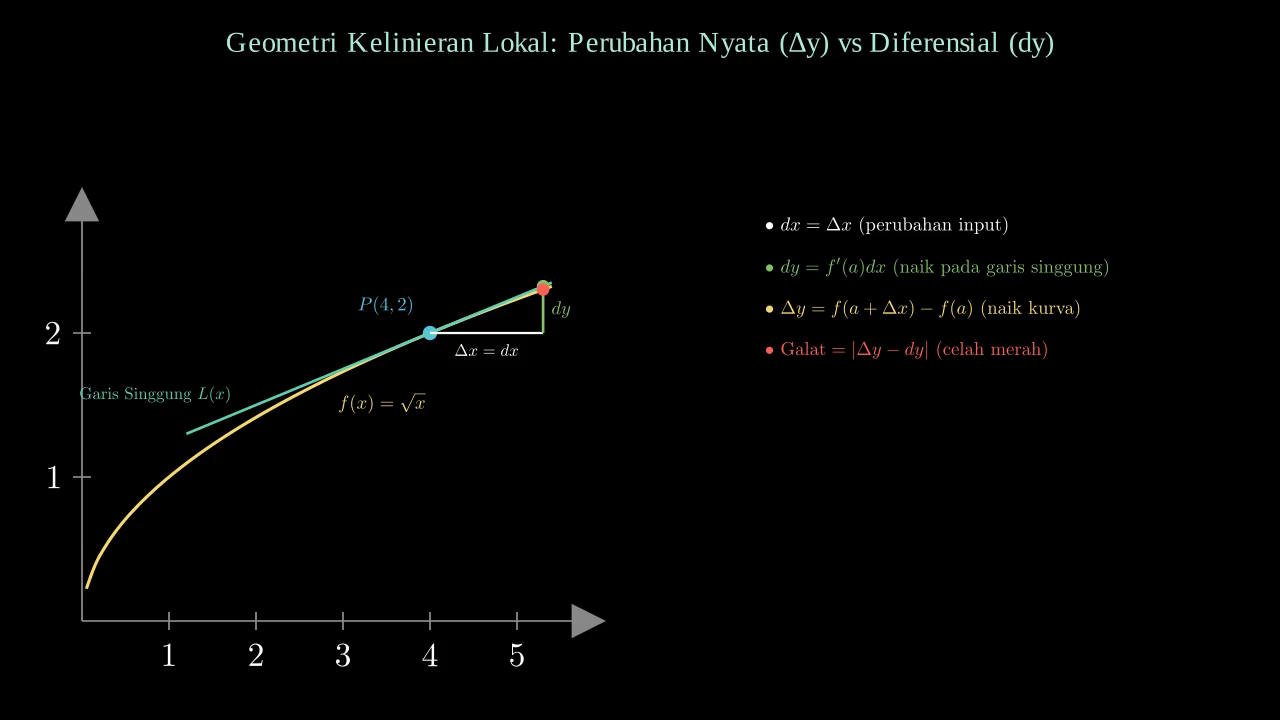
\includegraphics[height=0.55\textheight]{keyframe_diferensial.png}%
    }{DifferentialsApproximationScene.ogv}
    
    \vspace{0.2cm}
    \href{file:DifferentialsApproximationScene.mp4}{%
        \beamergotobutton{\normalsize $\blacktriangleright$ Putar Video (\texttt{DifferentialsApproximationScene.mp4})}%
    }
    
    \vspace{0.15cm}
    {\scriptsize \textit{Klik poster untuk memutar langsung di Pympress/Okular, atau klik tombol untuk membuka di MPV/VLC.}}
\end{frame}

% -------------------------------------------------------------
% Slide 5: Kristalisasi Matematis: Linierisasi & Diferensial
% -------------------------------------------------------------
\begin{frame}{Kristalisasi Formal: Linierisasi $L(x)$ dan Diferensial $dy$}
    \begin{columns}[T]
        \begin{column}{0.48\textwidth}
            \begin{block}{Definisi: Linierisasi Lokal $L(x)$}
                Jika $f$ terturunkan di $x = a$, persamaan garis singgung mendefinisikan \textbf{fungsi hampiran linier}:
                \[
                    \mathbf{L(x) = f(a) + f'(a)(x - a)}
                \]
                Untuk nilai $x$ di sekitar $a$:
                \[
                    \mathbf{f(x) \approx L(x)}
                \]
            \end{block}

            \begin{exampleblock}{Intisari Geometris}
                Di sekitar titik $a$, kurva lengkung $f(x)$ digantikan oleh fungsi linear derajat satu $L(x)$ yang mudah dievaluasi.
            \end{exampleblock}
        \end{column}

        \begin{column}{0.48\textwidth}
            \begin{block}{Notasi Diferensial Leibniz}
                Misalkan $y = f(x)$ adalah fungsi terturunkan:
                \begin{itemize}
                    \item $dx = \Delta x$ adalah bilangan riil sembarang.
                    \item Diferensial $dy$ didefinisikan sebagai:
                    \[
                        \mathbf{dy = f'(x)\,dx}
                    \]
                \end{itemize}
            \end{block}

            \begin{alertblock}{Rumus Hampiran Nilai Baru}
                Karena $\Delta y \approx dy$:
                \[
                    \mathbf{f(a + \Delta x) \approx f(a) + dy = f(a) + f'(a)\Delta x}
                \]
                Identik dengan evaluasi linierisasi $L(a + \Delta x)$!
            \end{alertblock}
        \end{column}
    \end{columns}
\end{frame}

% -------------------------------------------------------------
% Slide 6: Analisis Galat (Error Analysis)
% -------------------------------------------------------------
\begin{frame}{Analisis Galat: Mutlak, Relatif, dan Persentase}
    Dalam sains dan rekayasa, diferensial digunakan untuk menaksir perambatan galat pengukuran:

    \vspace{0.15cm}
    \begin{columns}[T]
        \begin{column}{0.32\textwidth}
            \begin{block}{1. Galat Mutlak}
                Besaran selisih antara aproksimasi dan nilai sebenarnya:
                \[
                    \text{Galat Mutlak} \approx |\mathbf{dy}|
                \]
                \[
                    |\Delta y| \approx |f'(x)\,dx|
                \]
                {\scriptsize \textit{Memiliki satuan yang sama dengan variabel $y$.}}
            \end{block}
        \end{column}

        \begin{column}{0.32\textwidth}
            \begin{block}{2. Galat Relatif}
                Perbandingan besar galat terhadap total besaran:
                \[
                    \text{Galat Relatif} \approx \left| \frac{\mathbf{dy}}{\mathbf{y}} \right|
                \]
                \[
                    \left| \frac{\Delta y}{y} \right| \approx \left| \frac{f'(x)\,dx}{f(x)} \right|
                \]
                {\scriptsize \textit{Besaran tanpa dimensi (mencerminkan presisi).}}
            \end{block}
        \end{column}

        \begin{column}{0.32\textwidth}
            \begin{block}{3. Galat Persentase}
                Galat relatif dinyatakan dalam persen (\%):
                \[
                    \text{Galat } \% \approx \left| \frac{\mathbf{dy}}{\mathbf{y}} \right| \times 100\%
                \]
                \vspace{0.15cm}
                {\scriptsize \textit{Standar spesifikasi toleransi alat industri.}}
            \end{block}
        \end{column}
    \end{columns}
\end{frame}

% -------------------------------------------------------------
% Slide 7: Contoh Soal 1: Hampiran Nilai Fungsi
% -------------------------------------------------------------
\begin{frame}{Contoh Soal 1: Menaksir Nilai Fungsi Tanpa Kalkulator}
    \begin{columns}[T]
        \begin{column}{0.48\textwidth}
            \begin{block}{Contoh A: Taksirlah Nilai $\sqrt{4.08}$}
                \begin{itemize}
                    \item \textbf{Model}: $f(x) = \sqrt{x}$, titik acuan $a = 4$
                    \item $f(4) = \sqrt{4} = 2$
                    \item $f'(x) = \frac{1}{2\sqrt{x}} \implies f'(4) = \frac{1}{4} = 0.25$
                    \item $dx = 4.08 - 4 = 0.08$
                    \item $dy = f'(4)\,dx = 0.25 \times 0.08 = \mathbf{0.02}$
                    \item $\sqrt{4.08} \approx 2 + 0.02 = \mathbf{2.02}$
                \end{itemize}
                \vspace{0.05cm}
                {\scriptsize \textit{Nilai kalkulator: $2.019901...$ (galat $< 10^{-4}$)}}
            \end{block}
        \end{column}

        \pause
        \begin{column}{0.48\textwidth}
            \begin{exampleblock}{Contoh B: Taksirlah Nilai $\cos(29^\circ)$}
                \textbf{Penting:} Sudut wajib diubah ke satuan radian!
                \begin{itemize}
                    \item $a = 30^\circ = \frac{\pi}{6}\text{ rad} \implies \cos\left(\frac{\pi}{6}\right) = \frac{\sqrt{3}}{2} \approx 0.8660$
                    \item $dx = 29^\circ - 30^\circ = -1^\circ = -\frac{\pi}{180}\text{ rad}$
                    \item $f'(x) = -\sin x \implies f'\left(\frac{\pi}{6}\right) = -0.5$
                    \item $dy = (-0.5)\left(-\frac{\pi}{180}\right) = \frac{\pi}{360} \approx +0.0087$
                    \item $\cos(29^\circ) \approx 0.8660 + 0.0087 = \mathbf{0.8747}$
                \end{itemize}
                \vspace{0.05cm}
                {\scriptsize \textit{Nilai kalkulator: $0.874619...$ (galat $< 10^{-4}$)}}
            \end{exampleblock}
        \end{column}
    \end{columns}
\end{frame}

% -------------------------------------------------------------
% Slide 8: Contoh Soal 2: Perambatan Galat Pengukuran Fisika
% -------------------------------------------------------------
\begin{frame}{Contoh Soal 2: Perambatan Galat Pengukuran Fisika}
    \textbf{Masalah}: Jari-jari bola diukur $r = 10\text{ cm}$ dengan batas galat pengukuran $\pm 0.1\text{ cm}$ (galat $1\%$). Taksirlah galat maksimum pada perhitungan volume bola $V = \frac{4}{3}\pi r^3$.

    \vspace{0.1cm}
    \pause
    \begin{columns}[T]
        \begin{column}{0.48\textwidth}
            \begin{block}{1. Taksiran Galat Mutlak}
                Diferensialkan $V = \frac{4}{3}\pi r^3$ terhadap $r$:
                \[
                    \frac{dV}{dr} = 4\pi r^2 \implies \mathbf{dV = 4\pi r^2\,dr}
                \]
                Substitusi $r = 10$ dan $|dr| \le 0.1$:
                \[
                    |dV| \le 4\pi (10)^2 (0.1) = 40\pi \approx \mathbf{125.66\text{ cm}^3}
                \]
            \end{block}
        \end{column}

        \begin{column}{0.48\textwidth}
            \begin{exampleblock}{2. Taksiran Galat Relatif \& Persentase}
                Bagi diferensial $dV$ dengan rumus volume $V$:
                \[
                    \frac{dV}{V} = \frac{4\pi r^2\,dr}{\frac{4}{3}\pi r^3} = \mathbf{3 \left(\frac{dr}{r}\right)}
                \]
                Substitusi galat relatif jari-jari $\frac{dr}{r} = \frac{0.1}{10} = 0.01$:
                \[
                    \text{Galat Relatif} \approx 3 \times 0.01 = \mathbf{0.03}
                \]
                \[
                    \text{Galat Persentase} \approx 0.03 \times 100\% = \mathbf{3\%}
                \]
                {\scriptsize \textit{Galat volume adalah 3 kali lipat galat radius!}}
            \end{exampleblock}
        \end{column}
    \end{columns}
\end{frame}

% -------------------------------------------------------------
% Slide 9: Latihan Mandiri & Rangkuman
% -------------------------------------------------------------
\begin{frame}{Latihan Mandiri \& Rangkuman Materi}
    \begin{columns}[T]
        \begin{column}{0.48\textwidth}
            \begin{block}{Latihan 1: Hampiran Akar Pangkat Tiga}
                Gunakan diferensial untuk menghampiri nilai $\sqrt[3]{28}$.\\
                \textit{(Petunjuk: Ambil fungsi $f(x) = x^{1/3}$, titik acuan kubik terdekat $a = 27$, sehingga $dx = 1$.)}
            \end{block}

            \begin{block}{Latihan 2: Pemuaian Termal Pelat Logam}
                Sebuah pelat logam bujur sangkar dengan sisi $x = 20\text{ cm}$ dipanaskan sehingga panjang sisinya bertambah sebesar $0.04\text{ cm}$.
                Taksirlah pertambahan luas pelat menggunakan diferensial $dA$, serta tentukan galat persentasenya!
            \end{block}
        \end{column}

        \begin{column}{0.48\textwidth}
            \begin{alertblock}{Rangkuman Inti Subtopik 2.9}
                \begin{itemize}
                    \item \textbf{Linierisasi}: $L(x) = f(a) + f'(a)(x - a)$.
                    \item \textbf{Diferensial}: $dy = f'(x)\,dx$.
                    \item \textbf{Hampiran Nilai}: $f(a + \Delta x) \approx f(a) + dy$.
                    \item \textbf{Perambatan Galat}: Galat relatif $\frac{dy}{y} = \frac{f'(x)dx}{f(x)}$. Jika $y = C x^n$, maka $\frac{dy}{y} = n \frac{dx}{x}$.
                \end{itemize}
            \end{alertblock}

            \vspace{0.15cm}
            \centering
            {\small \textbf{Selamat Belajar \& Sukses UTS MA1101!}}\\
            {\scriptsize Fakultas Matematika dan Ilmu Pengetahuan Alam --- ITB}
        \end{column}
    \end{columns}
\end{frame}

\end{document}
